%!TEX root = index.tex
\chapter{Analises}
\label{cha:analises}

\section{Samsung}

A partir de conversas com Luís Guilherme Selber, responsável pela operação do Laboratório Ocean, obtivemos a seguinte análise:

\begin{figure}[H]
\caption{Análise do Ocean - Samsung}
\centerline{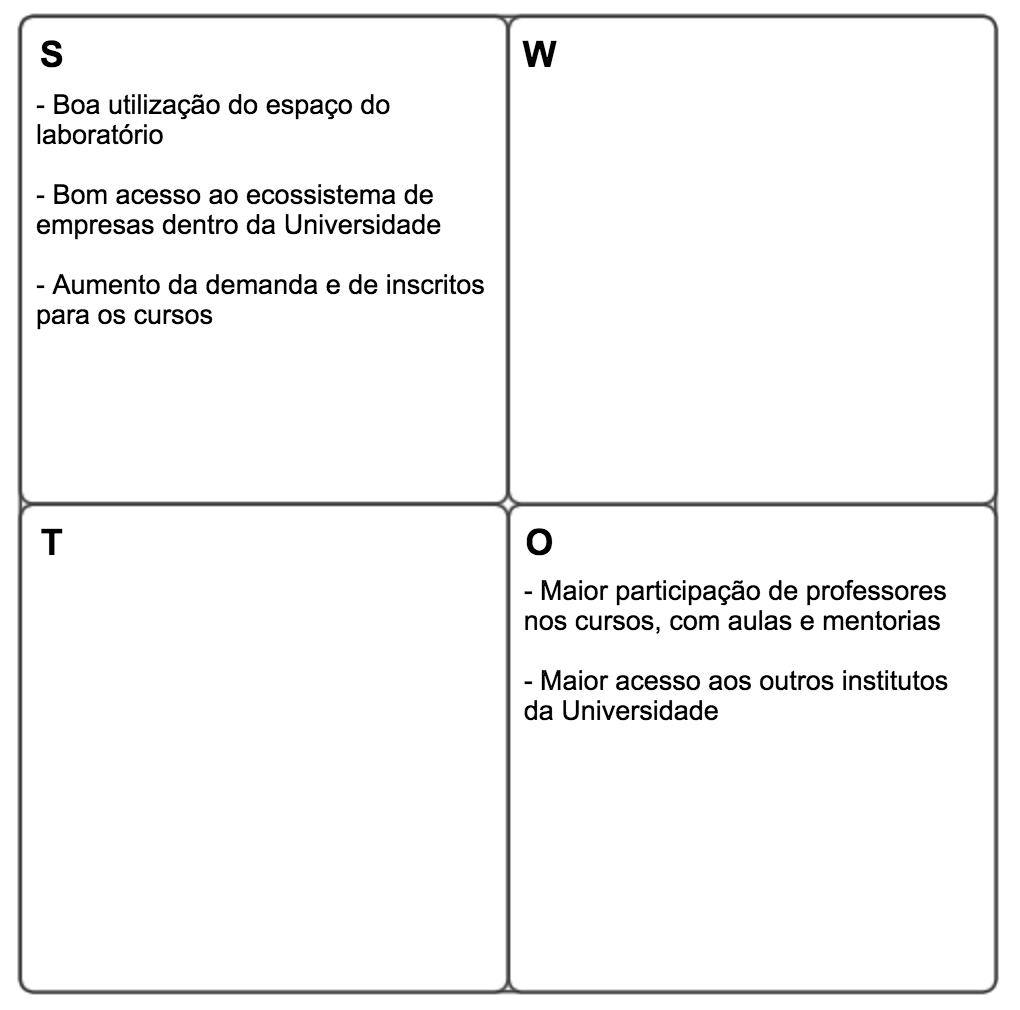
\includegraphics[scale=0.75]{img/samsungswot}}
\label{fig:swotsamsung}
\caption* {Fonte: Elaborado pelo próprio autor}
\end{figure}

A ausência de fraquezas e ameaças se dá - segundo o entrevistado - pelo fato de o projeto estar em uma fase inicial. Não há formalidades estabelecidas como reuniões periódicas, quando é necessário conversar sobre algo é fácil encontrar um professor no corredor ou em sua sala, portanto as interações se limitam às necessidades de um ou outro, sem conflitos até o momento. A própria gestão de uso do Laboratório para as atividades de cada instituição não gera conflitos pois as necessidades de uso do laboratório por cada parte já foram claramente estabelecidas nas reuniões iniciais de fechamento do projeto.

Em relação aos pontos fortes, destaca-se o fato de o laboratório sofrer uma mudança muito positiva devido à mudança de localidade para dentro da universidade. A presença do laboratório dentro do PRO mudou completamente a utilização do laboratório, que agora é ocupado das 08 da manhã até as 22 da noite de segunda a sexta, fato que não acontecia na Faria Lima. Quando na Av. Brigadeiro Faria Lima, a Samsung exercia um papel ativo de sediar eventos próprios ou externos com o intuito de divulgar e preencher o espaço do laboratório. Tudo isso porque mais pessoas utilizando o espaço ajuda a divulgar mais o programa e os cursos oferecidos pelo laboratório. Não obstante, além dos próprios cursos dados pelo laboratório, ainda existe um custo com equipamentos e internet que não deveria existir em vão.

Outra grande vantagem de estar dentro da universidade consiste no fato de a USP ser um ecossistema de parcerias com diversas empresas. Dentro desse meio, a Samsung ganha expande sua rede de contatos com outras empresas, já tendo provido até o momento reuniões com outras grandes empresas do mercado nacional.

O último ponto forte mencionado foi o aumento de demanda pelos cursos básicos e intensivos, houve um grande aumento principalmente por alunos da universidade. A proximidade com o NEU e a POLI permite uma divulgação muito mais fácil do laboratório na universidade.

Em relação às oportunidades, a Samsung vê como maiores oportunidades de melhoria uma maior participação de professores nos cursos do laboratório, seja através de aulas ou mentorias. Acredita-se que exista uma sinergia muito bom entre a academia e empresa no sentido de prender a atenção e incentivar os alunos dos cursos a buscarem mais conhecimento nas suas áreas de interesse.

Também acredita-se que possa haver uma adesão maior aos cursos e ao próprio dia a dia do laboratório por parte de outras instituições da Universidade. Tanto a FEA quanto o IME por suas formações ligadas ao empreendedorismo e ao desenvolvimento mostram ser muito compatíveis com os programas oferecidos pelo Ocean, entretanto a grande maioria de adeptos vêm da Escola Politécnica.

\section{PRO}

\begin{figure}[H]
\caption{Análise do Ocean - PRO}
\centerline{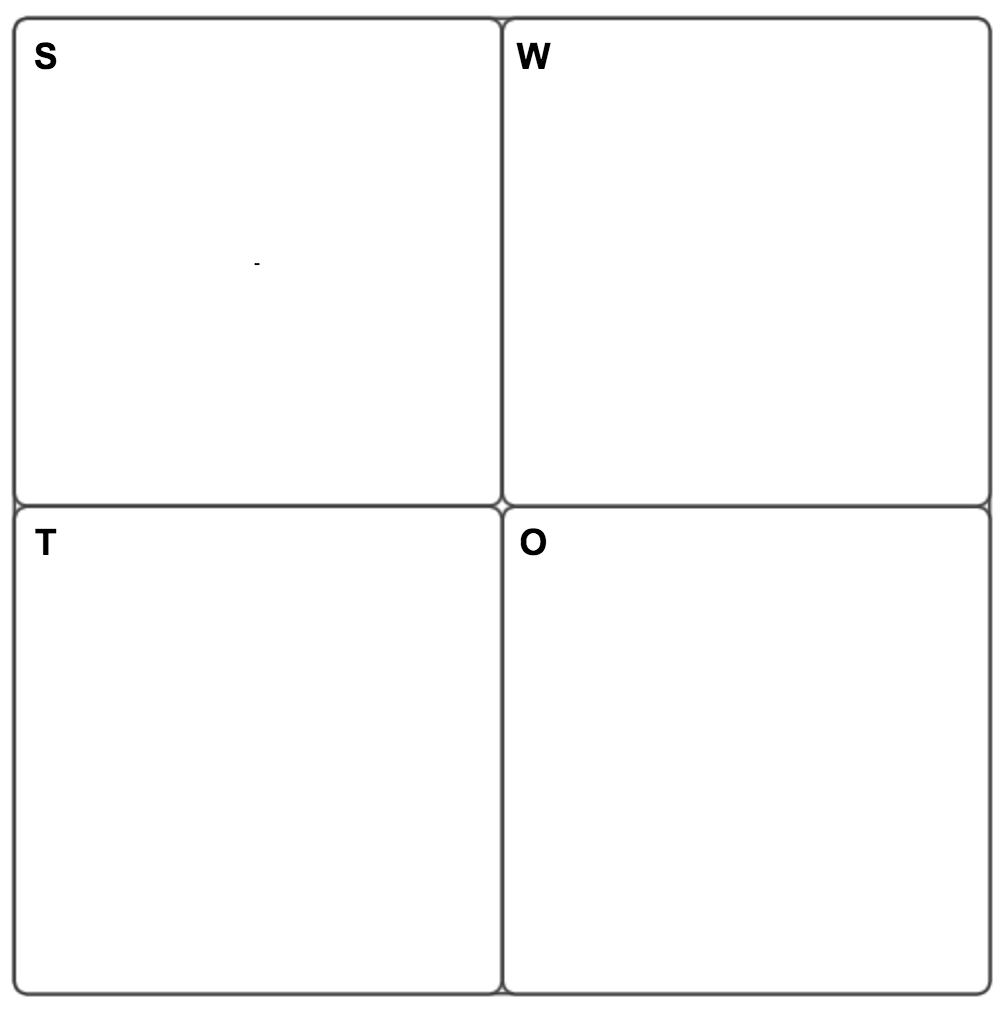
\includegraphics[scale=0.75]{img/generalswot}}
\label{fig:swotpro}
\caption* {Fonte: Elaborado pelo próprio autor}
\end{figure}

\section{NEU}

\begin{figure}[H]
\caption{Análise do Ocean - NEU}
\centerline{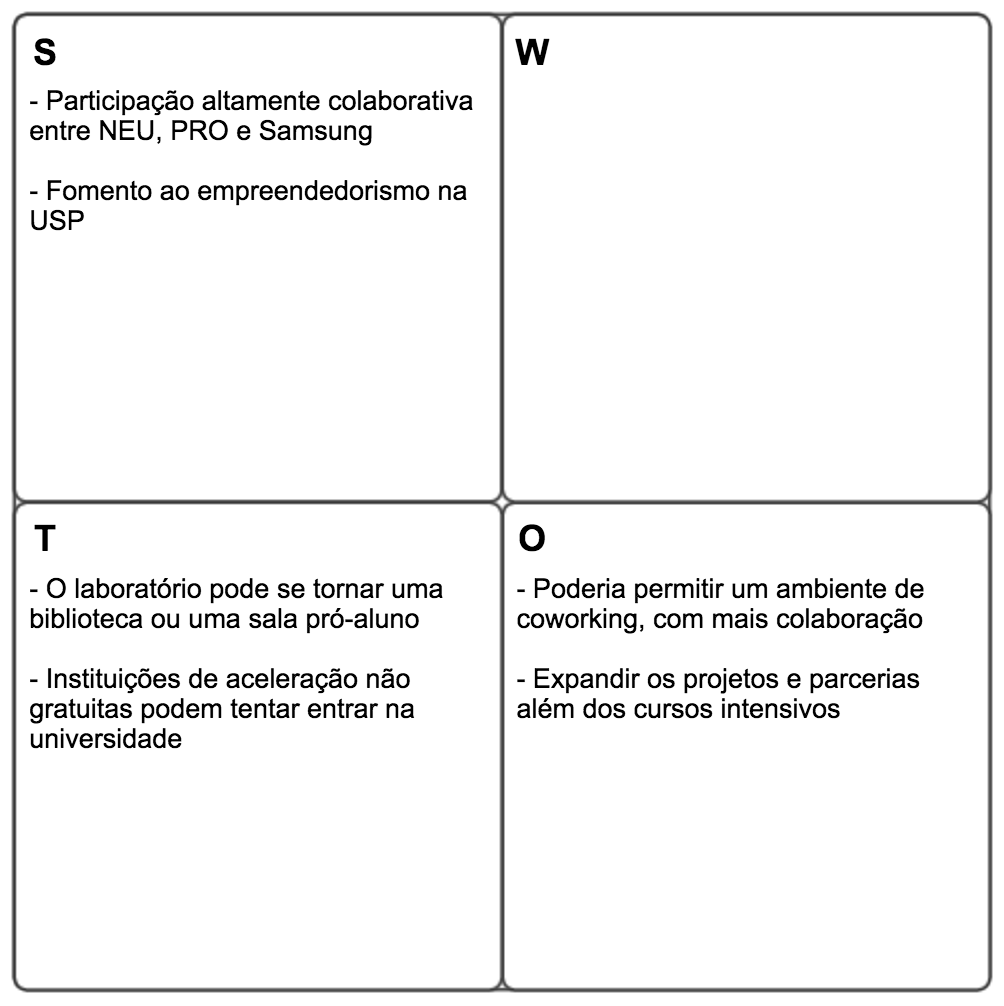
\includegraphics[scale=0.75]{img/neuswot}}
\label{fig:swotneu}
\caption* {Fonte: Elaborado pelo próprio autor}
\end{figure}

Segundo Juliana Uechi, atual responsável pelo funcionamento do NEU, a presença do Ocean por si só já contribui com o fomento à cultura de empreendedorismo dentro da Universidade, principal objetivo do NEU. Isso porque ainda existe uma carência de motivação pelo empreendedorismo, ainda mais em tempos de crise, a qual encontra no Ocean uma ferramenta gratuita com suporte à pré-aceleração de empresas. 

Atualmente existe uma colaboração ativa entre NEU, PRO e Samsung, principalmente em relação ao atual módulo de curso intensivo do laboratório, que envolve participação de todas as partes. De forma geral, a Samsung é responsável pelo acompanhamento do programa e pela capacitação, e o NEU e o PRO utilizam de suas conexões para trazer mentores às empresas participantes, normalmente ex-alunos que abriram as próprias empresas. Tais colaborações poderiam, segundo Juliana, ir além da participação nos cursos intensivos, porém a agenda de ambas as instituições encontra-se lotada

Em relação à infraestrutura do laboratório, o NEU acredita que o uso do laboratório é subutilizado quando cursos não estão acontecendo. O cenário atual de funcionamento é similar ao de uma biblioteca ou uma sala pró-aluno, onde alunos vão com tarefas individuais ou materiais de estudo, o que é de certa forma redundante pois já há uma biblioteca no departamento. Como uma frente de desenvolvimento e empreendedorismo, poderia haver mais espaço para \textit{coworking} e atividades colaborativas dentro do laboratório. Que fosse uma sala que gerasse valor através da discussão, não da absorção individual, que é igualmente importante, mas a biblioteca seria uma lugar mais adequado para esse tipo de atividade.

Por fim, é ressaltado a sinergia entre empresas que colaboram com o fomento à cultura de empreendedorismo, considerando que por mais que compartilhem o relacionamento com \textit{startups} via pré-aceleração, os alunos precisam ser motivados através de métodos diferentes. E pensando sempre no aluno e nas suas futuras empresas, um ambiente com diversas instituições de fomento ao empreendedorismo e aceleração, evita a entrada na universidade de instituições não-gratuitas, seja através de inscrição nos cursos ou via equity das empresas.

\section{Alunos}

\begin{figure}[H]
\caption{Análise do Ocean - Alunos}
\centerline{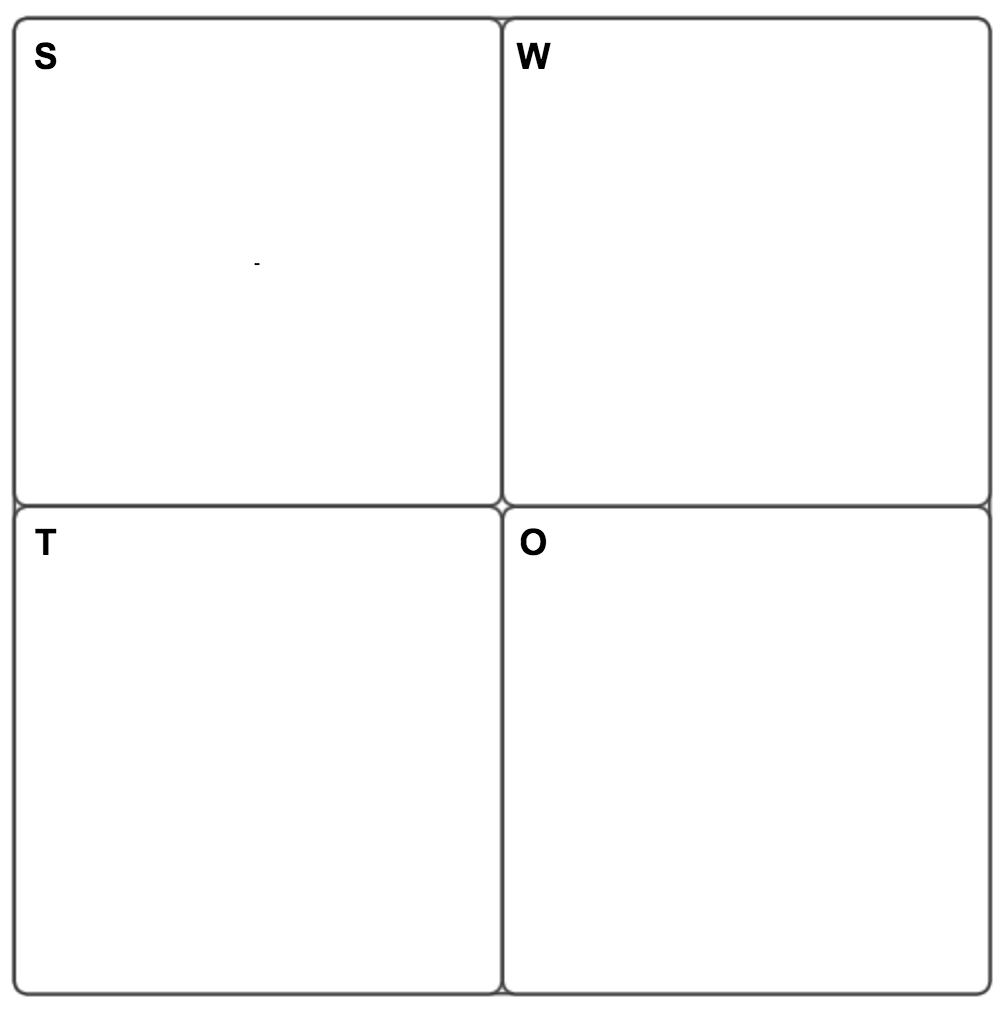
\includegraphics[scale=0.75]{img/generalswot}}
\label{fig:swotalunos}
\caption* {Fonte: Elaborado pelo próprio autor}
\end{figure}

\section{Cursistas}

Em relação aos cursistas de cursos básicos, a primeira questão curiosa é o fato de o item de resposta de feedback sobre a localização ter piorado após a migração para dentro da USP.

\begin{figure}[h]
\caption{Análise do Ocean - Cursistas}
\centerline{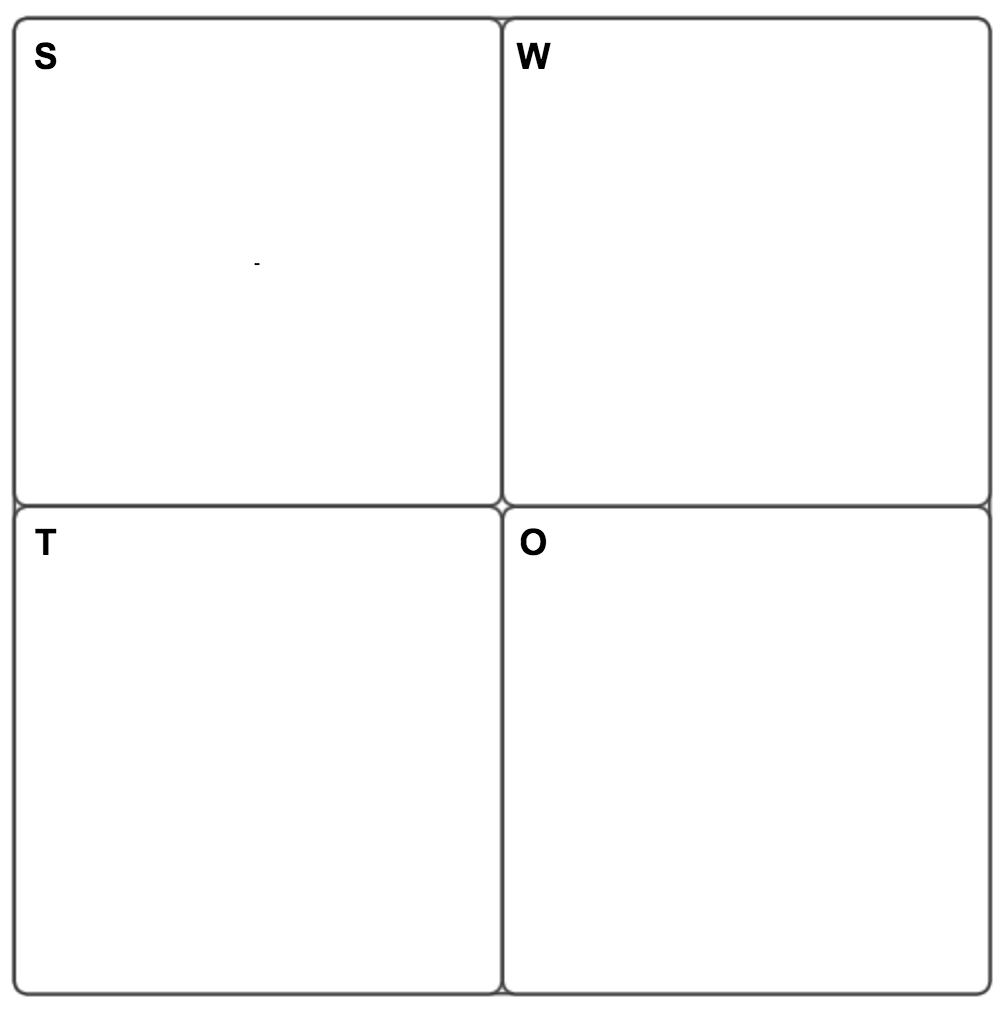
\includegraphics[scale=0.75]{img/generalswot}}
\label{fig:swotcursistas}
\caption* {Fonte: Elaborado pelo próprio autor}
\end{figure}